\problem{15}
%We considered the virial expansion for non-ideal classical gases
%in the previous homework.
This problem will demonstrate how the behavior of 
an ideal quantum gas
compares to that of a classical gas.
We focus on chemical potential and pressure,
noting that all other properties can be derived from $\mu$ and $p$.
Our goal is to derive virial expansions describing
ideal Fermions and Bosons.

\smallskip \subp
Much of what we do in statistical mechanics is counting.
When we compute entropy in the microcanonical ensemble,
we count microstates.
Similarly, the canonical and grand canonical
partition functions are calculated
by counting Boltzmann factors.
%Recall from class that we use 
%a permutation factorial ($1/N!$)
%to account for indistinguishability, and 
%a factor of $h^3$ to non-dimensionalize
%integration over phase volume.
Show that the following counting expressions
for translational degrees of freedom
in a quantum ideal gas are identical:
\[
\sum_{{\bf n} = 0}^\infty \, \quad = \quad 
%\frac{V}{h^3} \int_{-\infty}^{\infty}\dd{\bf p} \quad,\quad
\frac{V}{(2\pi)^3} \int_{-\infty}^{\infty}\dd{\bf k} \quad = \quad
\left(\frac{V}{\Lambda^3}\right) \frac{2}{\sqrt\pi} \int_0^\infty
  \!\dd x\, x^{1/2}
\quad .
\]
Above,
${\bf n} \equiv \{n_x,n_y,n_z\}$,
${\bf k} = \frac{\pi}{L} {\bf n}$,
$\epsilon = \frac{\hbar^2 |{\bf k}|^2}{2 m}$,
$x = \frac{\epsilon}{\kT}$,
and $\Lambda$ is the thermal de~Broglie wavelength. 
You may assume whatever you are summing over
depends on ${\bf n}$ only through $\epsilon$. 
\solution{ \\
Reminder: translational energy levels 
for a quantum gas come from
the 3D particle in a box:
\[ E_{\bf n} 
= \frac{h^2 |{\bf n}|^2}{8 m L^2} 
= \frac{4 \hbar^2}{8 m} \left| \frac{\pi \bf{n}}{L} \right|^2 
= \frac{\hbar^2 |{\bf k}|^2}{2 m} = \epsilon \]
At high temperatures
(in the classical limit), we may assume that
translational energy levels are so closely spaced
that we can replace the summation over $n$ with an integral.
No normalization is required here because
$n$ is dimensionless. Since $\epsilon = \epsilon(|{\bf n}|^2)$
is even with respect to ${\bf n}$:
\[ \sum_{{\bf n} = 0}^\infty \approx
   \int_0^\infty \dd n_x 
   \int_0^\infty \dd n_y 
   \int_0^\infty \dd n_z 
 = \frac{1}{2^3} 
   \int_{-\infty}^\infty \dd n_x 
   \int_{-\infty}^\infty \dd n_y 
   \int_{-\infty}^\infty \dd n_z \]
Given that ${\bf k} = \frac{\pi}{L} {\bf n}$, 
we substitute in ${\bf n} = \frac{L}{\pi} {\bf k}$.
\[ \sum_{{\bf n} = 0}^\infty 
   \approx \frac{1}{2^3}
           \int_{-\infty}^\infty \frac{L}{\pi} \, \dd k_x 
           \int_{-\infty}^\infty \frac{L}{\pi} \, \dd k_y 
           \int_{-\infty}^\infty \frac{L}{\pi} \, \dd k_z
         = \frac{L^3}{(2\pi)^3} 
           \int_{-\infty}^{\infty} \dd {\bf k} \]
Here $L^3 \equiv V$ is the `box' volume.
It is understood that the rightmost integral
is shorthand for the three integrals over
$k_x$, $k_y$, and $k_z$. 
We have therefore shown that:
\[ \boxed{ \sum_{{\bf n} = 0}^\infty 
         = \frac{V}{(2\pi)^3} \int_{-\infty}^\infty \dd {\bf k} } \]
Assume that we are summing over a function that depends only
on $\epsilon = \epsilon(|{\bf k}|)$. 
Since $\epsilon$ depends only on the magnitude of ${\bf k}$,
we can change to spherical coordinates:
\[ \frac{V}{(2\pi)^3} \int_{-\infty}^{\infty} \dd {\bf k} 
 \equiv \frac{V}{(2\pi)^3}
   \int_{-\infty}^\infty \dd k_x 
   \int_{-\infty}^\infty \dd k_y 
   \int_{-\infty}^\infty \dd k_z
 = \frac{V}{(2\pi)^3} \int_0^\infty \dd |{\bf k}| 
    \, 4 \pi |{\bf k}|^2 \]
Recall $\Lambda \equiv \frac{h}{\sqrt{2\pi m \kT}}$ 
and $x \equiv \beta \epsilon$. 
Examining our definitions:
\[ x = \frac{\hbar^2}{2 m \kT} |{\bf k}|^2
     = \frac{h^2}{8 \pi^2 m \kT} |{\bf k}|^2
     = \frac{\Lambda^2}{4 \pi} |{\bf k}|^2 \]
Solve for $|{\bf k}|$ to get a conversion to $\dd x$:
\[   |{\bf k}| = \frac{2 \sqrt{\pi} x^{1/2}}{\Lambda} \quad \Rightarrow \quad
 \dd |{\bf k}| = \frac{\sqrt{\pi} x^{-1/2}}{\Lambda} \dd x \]
Substitute back in to get:
\begin{align*}
    \frac{V}{(2\pi)^3} \int_0^\infty \dd |{\bf k}| \, 
    4 \pi |{\bf k}|^2 f(|{\bf k}|) 
 &= \frac{V}{(2\pi)^3} \int_0^\infty \dd x \, 
    \left( \frac{\sqrt{\pi} x^{-1/2}}{\Lambda} \right)
    \left( 4 \pi \times \frac{4 \pi x}{\Lambda^2} \right) f(x) \\
 &= \frac{V}{(2\pi)^3} \left( \frac{16 \pi^{5/2}}{\Lambda^3} \right) 
    \int_0^\infty \dd x \, x^{1/2} f(x) \\
 &= \left( \frac{V}{\Lambda^3} \right) \frac{2}{\sqrt{\pi}}
    \int_0^\infty \dd x \, x^{1/2} f(x)
\end{align*}
Thus, we have shown:
\[ \boxed{ \sum_{{\bf n} = 0}^\infty 
         = \frac{V}{(2\pi)^3} 
           \int_{-\infty}^{\infty}\dd{\bf k} 
         = \left(\frac{V}{\Lambda^3}\right) \frac{2}{\sqrt\pi} 
           \int_0^\infty \!\dd x\, x^{1/2} } \]
}


\smallskip \subp
Now consider ideal Bosons and Fermions.
%Use the equation of state for chemical potential
%\kh{confusing},
Using the Fermi-Dirac and Bose-Einstein occupation
numbers derived in class,
show that at high temperature, 
the chemical potential $\mu$ is given by
\[
\mu = \kT \left( \ln\left(\rho \Lambda^3\right) \mp
  \frac{\rho \Lambda^3}{2^{3/2}} +
  \cdots \right) ,
\]
in which $\rho = N/V$ is the particle number density.
The top and bottoms signs are for Bosons (-) 
and Fermions (+), respectively.
The first term is the chemical potential for classical particles.
The second term is the lowest order quantum correction. 
{\bf Hint:} Find a series expansion for 
$\rho \Lambda^3$ by Taylor expanding 
$u \equiv \lambda e^{-\beta \epsilon_i}$,
where $\lambda \equiv e^{\beta \mu}$.
Recall that $\lambda = \sum_{n=1} a_n \rho^n$ 
can be obtained by inverting 
$\rho \Lambda^3 = \sum_{n=1} b_n \lambda^n$
(similar to HW5). 
\solution{ 
\[ N = \sum_i \ave{n_i}
 = \sum_{{\bf n}=0}^{\infty} 
   \frac{1}{e^{\beta(\epsilon_i - \mu)} \mp 1}
 = \sum_{{\bf n}=0}^{\infty} \frac{1}{u^{-1} \mp 1}
 = \sum_{{\bf n}=0}^{\infty} \frac{u}{1 \mp u} \]
The top sign is for bosons
and the bottom sign is for fermions.
Now Taylor expand $\frac{1}{1 \mp u}$:
\[ \frac{1}{1 \mp u}  
 = \sum_{j=0}^\infty (\pm u)^j
 = 1 \pm u + \ldots \]
You may ask why we can treat 
$u \equiv e^{-\beta(\epsilon_i - \mu)}$
as a small parameter even though $\beta \rightarrow 0$
in the classical limit.
Recall from class that $\mu_{\rm classic} \propto -T \ln T$.
Therefore, $\lambda \equiv e^{\beta \mu} \rightarrow 0$
as $T \rightarrow \infty$, and so $u \ll 1$. 
Apply the result from part (a)
to convert the sum to an integral over $x$:
\[ N = \sum_{{\bf n}=0}^{\infty} \frac{u}{1 \mp u} \\
     = \left( \frac{V}{\Lambda^3} \right) \frac{2}{\sqrt{\pi}} 
       \int_0^\infty \! \dd x \, x^{1/2} 
       \left( u \pm u^2 + \ldots \right) \]
Now write $u$ in terms of $x$, 
i.e. $u \equiv  e^{-\beta(\epsilon_i - \mu)} = \lambda e^{-x}$:
\begin{align*}
 N &= \left( \frac{V}{\Lambda^3} \right) \frac{2}{\sqrt{\pi}} 
      \left[ \lambda   \int_0^\infty \dd x \, x^{1/2} e^{-x}
         \pm \lambda^2 \int_0^\infty \dd x \, x^{1/2} e^{-2x} 
           + \ldots \right] \\
   &= \left( \frac{V}{\Lambda^3} \right) \frac{2}{\sqrt{\pi}} 
      \left[ \frac{\sqrt{\pi} \lambda}{2} 
         \pm \frac{\sqrt{\pi} \lambda^2}{4\sqrt{2}} 
           + \ldots \right] \\
   &= \left( \frac{V}{\Lambda^3} \right)
      \left[ \lambda \left( 1 \pm \frac{\lambda}{2 \sqrt{2}} 
           + \ldots \right) \right]
\end{align*}
This lets us write a series expression for $\rho \Lambda^3$:
\[ \rho \Lambda^3 = \sum_{n=1} b_n \lambda^n
 = \lambda \left( 1 \pm \frac{\lambda}{2^{3/2}} + \ldots \right) \]
\[ b_1 = 1 \quad , \quad b_2 = \pm \frac{1}{2^{3/2}} \]
To reiterate, the top sign is for bosons and bottom sign is for fermions.
We would like to find $\lambda = \sum_{n=1} a_n (\rho \Lambda^3)^n$.
Invert the expression by substituting in 
$\rho \Lambda^3 = b_1 \lambda + b_2 \lambda^2 + \ldots$
\begin{align*}
  \lambda &= a_1 (\rho \Lambda^3) + a_2 (\rho \Lambda^3)^2 + \ldots 
           = a_1 (b_1 \lambda + b_2 \lambda^2 + \ldots) 
           + a_2 (b_1 \lambda + b_2 \lambda^2 + \ldots)^2 \\ 
          &= a_1 b_1 \lambda + (a_1 b_2 + a_2 b_1^2) \lambda^2 + \ldots
\end{align*}
Matching coefficients, we see that
$a_1 = b_1^{-1} = 1$ and $a_2 = -b_2$. Thus:
\[ \lambda \equiv e^{\beta \mu} 
 = \rho \Lambda^3 \left( a_1 + a_2 \rho \Lambda^3 + \ldots \right) 
 = \rho \Lambda^3 \left( 1 \mp \frac{\rho \Lambda^3}{2^{3/2}} 
                      + \ldots \right) \]
Take the logarithm of both sides,
then Taylor expand noting that $\rho \Lambda^3 \ll 1$
when $T$ is large:
\[ \beta \mu 
= \ln(\rho \Lambda^3)
+ \ln(1 \mp \frac{\rho \Lambda^3}{2^{3/2}} + \ldots) \approx
  \ln(\rho \Lambda^3) \mp \frac{\rho \Lambda^3}{2^{3/2}} + \ldots \]
This is precisely what we wanted to show!
\[ \boxed{ 
   \mu = \kT \left[ 
         \ln (\rho \Lambda^3) 
     \mp \frac{\rho \Lambda^3}{2^{3/2}} 
       + \ldots \right] } \]
The top (minus) sign is for bosons
and the bottom (plus) sign is for fermions.
}

\smallskip \subp
Using the equation of state for the pressure
of an ideal quantum gas derived in class,
show that an analogous expansion for pressure holds
at high temperature, i.e.,
$$
p = \rho \kT \left( 1 \mp \frac{\rho \Lambda^3}{2^{5/2}}
     + \cdots \right) .
$$
The second term is a correction to ideal gas behavior.
The coefficient $\mp \Lambda^3 / 2^{5/2}$
is the second virial coefficient for quantum gases.
It is negative for Bosons and positive for Fermions,
implying that, to first approximation,
non-interacting Bosons and Fermions behave like
ideal gases with weak attractive or repulsive interactions! 
%The factor $\rho\Lambda^3$ obviously tells us
%when the molecules can be treated classically.
\solution{\\
From the Lecture 12 notes
(top sign for Bosons, bottom sign for Fermions):
\[ pV = \kT \ln \Xi = \mp \kT \sum_i 
   \left[ \ln \left( 1 \mp \lambda
           e^{-\beta \epsilon_i} \right) \right] \]
We established in (b) that
$\lambda \equiv e^{\beta \mu} \ll 1$
in the high $T$ limit. 
Taylor expand the logarithm:
\[ p = \mp \frac{\kT}{V} \sum_i \left[ 
       \mp \lambda e^{-\beta \epsilon_i} 
         - \frac{\lambda^2 e^{-2\beta \epsilon_i}}{2}
         + \ldots \right] 
     = \frac{\kT}{V} \sum_i \left[ 
       \lambda e^{-\beta \epsilon_i} 
       \pm \frac{\lambda^2 e^{-2 \beta \epsilon_i}}{2}
       + \ldots \right] \]
Now let's get rid of the summation using 
the identity derived in part (a):
\begin{align*}
  p &= \left( \frac{\kT V}{\Lambda^3 V} \right)
       \frac{2}{\sqrt{\pi}} \int_0^\infty \dd x \, x^{1/2} 
       \left[ \lambda e^{-x} \pm \frac{\lambda^2 e^{-2x}}{2} 
            + \ldots \right] \\
    &= \left( \frac{\kT}{\Lambda^3} \right)
       \frac{2}{\sqrt{\pi}} \left[
       \frac{\lambda \sqrt{\pi}}{2}
       \pm \frac{\lambda^2 \sqrt{\pi}}{8\sqrt{2}} + \ldots \right] \\
    &= \left( \frac{\kT}{\Lambda^3} \right)
       \left[ \lambda \pm \frac{\lambda^2}{2^{5/2}} + \ldots \right]
\end{align*}
Substitute in
$\lambda = \rho \Lambda^3 
 \left(1 \mp \frac{\rho \Lambda^3}{2^{3/2}} + \ldots \right)$,
which we showed in part (b).
\begin{align*}
  p &= \frac{\kT}{\Lambda^3} \left[ \rho \Lambda^3 
       \left(1 \mp \frac{\rho \Lambda^3}{2^{3/2}} + \ldots \right)
   \pm \frac{\rho^2 \Lambda^6}{2^{5/2}}
       \left(1 \mp \frac{\rho \Lambda^3}{2^{3/2}} + \ldots \right)^2
     + \ldots \right] \\
    &= \rho \kT \left[ 1 \mp \frac{\rho \Lambda^3}{2^{3/2}} 
                         \pm \frac{\rho \Lambda^3}{2^{5/2}} 
                           + \ldots \right]
     = \rho \kT \left[ 1 \mp \left( \frac{2 \rho \Lambda^3}{2^{5/2}} 
                                   -\frac{\rho \Lambda^3}{2^{5/2}} \right)
                           + \ldots \right] \\
    &= \rho \kT \left[ 1 \mp \frac{\rho \Lambda^3}{2^{5/2}} + \ldots \right]
\end{align*}
Finally there! Thus, to second order, 
the virial expansion for an ideal quantum gas is:
\[ \boxed{ p = \rho \kT 
   \left[  1 \mp \frac{\rho \Lambda^3}{2^{5/2}} + \ldots \right] } \]
}

\bigskip
\problem{10}
Chemical reaction equilibrium can be analyzed statistically.
Consider the ammonia synthesis reaction:
\[ \ce{N2(g) + 3H2(g) <--> 2NH3(g)} \]
Assume all gas molecules can be treated
as classical ideal gases.
Let $g_{\rm N_2}$, $g_{\rm H_2}$,
and $g_{\rm NH_3}$
denote the free energy
due to the internal degrees of freedom
(rotational and vibrational modes)
of each species.

\smallskip \subp
Using the canonical ensemble
$(N_{\rm N_2}, N_{\rm H_2}, N_{\rm NH_3}, V, T)$,
show that the Helmholtz free energy is:
\begin{align*}
F(N,V,T)
 = \sum_{X={\rm N_2, H_2, NH_3}}
    N_X \kT \left[ \ln\left( \frac{N_X \Lambda_X^3}{V e} \right)
    + \frac{g_{X}}{\kT} \right] .
%F &= N_{\rm N_2} \kT \left[ \ln\left( \frac{N_{\rm N_2}\Lambda_{\rm N_2}^3}{V e} \right) + g_{\rm N_2} \right]
%+
%N_{\rm H_2} \kT \left[ \ln\left( \frac{N_{\rm H_2}\Lambda_{\rm H_2}^3}{V e} \right) + g_{\rm H_2} \right] \\
%& \qquad \qquad +
%N_{\rm NH_3} \kT \left[ \ln\left( \frac{N_{\rm NH_3}\Lambda_{\rm NH_3}^3}{V e} \right) + g_{\rm NH_3} \right]
%]
\end{align*}
\solution{ 
We generalize our results for the classical ideal gas (from lecture)
to a multi-component system:
\[ Q(N,V,T) = \prod_X \frac{q_X^{N_X}}{N_X!} 
 = \frac{ q^N_{\ce{N2}} q^N_{\ce{H2}} q^N_{\ce{NH3}} }
        { N_{\ce{N2}}! N_{\ce{H2}}! N_{\ce{NH3}}! } \]
Helmholtz free energy is directly related to Q:
\[ F = -\kT \ln Q = -\kT \ln \left[ \prod_X \frac{q^{N_X}}{N_X!} \right]
     = -\kT \sum_X \left[ N_X \ln q_X 
       -N_X \ln \left( \frac{N_X}{e} \right) \right] \]
We have applied the Stirling approximation above.
Note the logarithm of a product is a sum.
Let's take a closer look at $q_X = q_t q_r q_v$:
\[ \ln q_X = \ln q_t + \ln q_r + \ln q_v 
           = \ln \left( \frac{V}{\Lambda_X^3} \right) - \frac{g_X}{\kT} \]
Here, $g_X \equiv -\kT \ln (q_r q_v)$
accounts for internal (non-translational) 
degrees of freedom.
\[ F = \sum_X -N_X \kT \left[ 
       \ln \left( \frac{V}{\Lambda_X^3} \right)
     - \frac{g_X}{\kT} - \ln \left( \frac{N_X}{e} \right) \right]  \]
\[ \boxed{ F = \sum_X N_X \kT \left[ \ln \left( 
          \frac{N_X \Lambda_X^3}{V e} \right) + \frac{g_X}{\kT} \right]  } \]
\newpage
}

\smallskip \subp
Denote the extent of reaction as $n$,
which is positive if the reaction
proceeds forwards, and negative if 
the reaction proceeds backwards.
Reaction equilibrium is reached
when free energy is minimized,
i.e.  $\pdc{F}{n}{V,T} = 0$.
Show that equilibrium is given
by the following condition: 
\[ \nu_{\rm N_2} \mu_{\rm N_2} + 
   \nu_{\rm H_2} \mu_{\rm H_2} + 
   \nu_{\rm NH_3} \mu_{\rm NH_3} = 0, \]
where
$\nu_{\rm N_2} = -1$,
$\nu_{\rm H_2} = -3$, and
$\nu_{\rm NH_3} = 2$ are 
stoichiometric coefficients.
\solution{\\
Mass must be conserved:
\[ \dd n = \frac{\dd N_{\ce{N2}}}{\nu_{\ce{N2}} }
         = \frac{\dd N_{\ce{H2}}}{\nu_{\ce{H2}} }
         = \frac{\dd N_{\ce{NH3}}}{\nu_{\ce{NH3}} } \]
This indicates that $\nu_X = \frac{\dd N_X}{\dd n}$.
Write the minimization condition
for $F(N_{\rm N_2}, N_{\rm H_2}, N_{\rm NH_3}, V, T)$:
\begin{align*}
 \pdc{F}{n}{V,T}
 &= \frac{\dd N_{\ce{N2}}}{\dd n}
    \pdc{F}{N_{\ce{N2}}}{N_{\bf other},V,T}
  + \frac{\dd N_{\ce{H2}}}{\dd n}
    \pdc{F}{N_{\ce{H2}}}{N_{\bf other},V,T}
  + \frac{\dd N_{\ce{NH3}}}{\dd n}
    \pdc{F}{N_{\ce{NH3}}}{N_{\bf other},V,T} \\[2mm]
 &= \nu_{\ce{N2}}  \mu_{\ce{N2}}
  + \nu_{\ce{H2}}  \mu_{\ce{H2}}
  + \nu_{\ce{NH3}} \mu_{\ce{NH3}} = 0
\end{align*}
Since, by definition, $\mu_X \equiv \pdc{F}{N_X}{N_{\bf other},V,T}$ .
Therefore, we have shown that:
\[ \boxed{ \nu_{\ce{N2}}  \mu_{\ce{N2}}
         + \nu_{\ce{H2}}  \mu_{\ce{H2}}
         + \nu_{\ce{NH3}} \mu_{\ce{NH3}} = 0 } \]
}

\smallskip \subp
Let us adopt the standard notation for concentration,
$[X] \equiv N_X / V$
($X = \rm N_2$, $\rm H_2$, or $\rm NH_3$).
Show that the condition from part~(b) yields
the following expression for law of mass-action.
\[
\frac{[{\rm NH_3}]^2}{[{\rm N_2}][\rm H_2]^3} = K_{\rm eq}
\equiv \left(\frac{\Lambda_{\rm N_2} \Lambda_{\rm H_2}^3}
       {\Lambda_{\rm NH_3}^2}\right)^3
  \exp\left(- \frac{2g_{\rm NH_3} -
  g_{\rm N_2} - 3 g_{\rm H_2}} {\kT} \right) .
\]
Note that the prefactor in $K_{\rm eq}$
has a weak temperature dependence
($\propto T^{-3}$).
\solution{\\
Begin by finding an expression for 
$\mu_X \equiv \pdc{F}{N_X}{N_{\bf other},V,T}$ :
\begin{align*}
\mu_X &= \kT \frac{\partial}{\partial N_X} 
         \left[ N_X \ln \left( \frac{N_X \Lambda_X^3}{V e} \right) 
              + \frac{N_X g_X}{\kT} \right] \\
      &= \kT \left[ \ln \left( \frac{N_X \Lambda_X^3}{V e} \right) 
                  + \frac{g_X}{\kT}
                  + \frac{N_X}{N_X} \right] \\
      &= \kT \left[ \ln \left( [X] \Lambda_X^3\right) + \frac{g_X}{\kT} \right]
\end{align*}
In general form, the equilibrium condition is given by:
\[ \sum_X \nu_X \mu_X = \kT \sum_X \nu_X 
   \left[ \ln \left( [X] \Lambda_X^3 \right) + \frac{g_X}{\kT} \right] = 0 \]
\[ -\sum_X \nu_X \ln \left( [X] \Lambda_X^3 \right) 
 =  \sum_X \nu_X \frac{g_X}{\kT} \]
For our system,
$\nu_{\rm N_2} = -1$,
$\nu_{\rm H_2} = -3$, and
$\nu_{\rm NH_3} = 2$.
\[   \ln \left( [\ce{N2}]  \Lambda_{\ce{N2}}^3  \right) 
   +3 \ln \left( [\ce{H2}]  \Lambda_{\ce{H2}}^3  \right)
   -2 \ln \left( [\ce{NH3}] \Lambda_{\ce{NH3}}^3 \right)
   =  \frac{- g_{\ce{N2}} - 3 g_{\ce{H2}} + 2 g_{\ce{NH3}} }{\kT} \]
\[ \ln \left[ \frac{ [\ce{N2}] [\ce{H2}]^3 }{ [\ce{NH3}]^2 }
   \left( \frac{ \Lambda_{\ce{N2}} \Lambda_{\ce{H2}}^3 }
   { \Lambda_{\ce{NH3}}^2 } \right)^3 \right] 
 = \frac{-g_{\ce{N2}} - 3 g_{\ce{H2}} + 2 g_{\ce{NH3}} }{\kT} \]
Take the exponential of both sides and do some minor rearranging to get:
\[ \boxed{ \frac{ [\ce{NH3}]^2 }{ [\ce{N2}] [\ce{H2}]^3 } 
 = \left( \frac{ \Lambda_{\ce{N2}} \Lambda_{\ce{H2}}^3 }
   { \Lambda_{\ce{NH3}}^2 } \right)^3
   \exp \left( -\frac{2 g_{\ce{NH3}} - g_{\ce{N2}} - 3g_{\ce{H2}} }{\kT} \right) } \]
}

\bigskip
\problem{25}
Myoglobin and hemoglobin are proteins that bind and
transport oxygen to cells and tissues.
Binding of oxygen molecules ($O_2$) occurs at heme groups
in the proteins; myoglobin has a single heme group, 
while hemoglobin has four heme groups corresponding
to four oxygen-binding sites.
In this problem, we will use a simple adsorption model 
(first developed by Linus Pauling)
to model oxygen binding in myoglobin and hemoglobin.
The binding of oxygen to a heme group is associated with 
a favorable energy $-\epsilon$.
For hemoglobin,
there is an additional favorable interaction energy $-\delta$ when
oxygen is bound to adjacent sites.  Thus, the total energy for
2 bound oxygens is $-2 \epsilon - \delta$, 
for 3 bound oxygens is $-3 \epsilon - 3 \delta$, etc.
The oxygen in the surrounding solution
has chemical potential $\mu = k_{B}T \ln(x) +\mu_{0}$, 
where $x$ is the oxygen concentration.

\begin{figure}[h]\centering
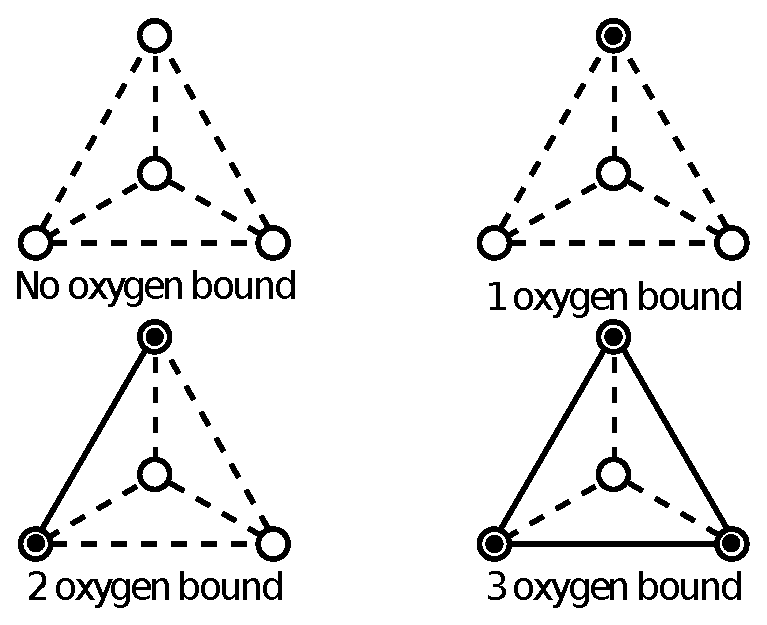
\includegraphics[width=0.4\textwidth,height=!]{hemoglobin}
\caption{\label{fig:hemoglobin}
Schematic of the Pauling model for oxygen binding to hemoglobin.}
\end{figure}

\smallskip\subp
Find the grand canonical partition function:
$\Xi_\text{m}$ for the single-site model of myoglobin.
\solution{ \\
We know $\Xi \equiv \sum_i \exp \left( \frac{-E_i + \mu N_i}{\kT} \right)$.
Write out all the states:
\begin{center}
 \begin{tabular}{||c|c|c||} 
 \hline
 $N_i$ & $E_i$ & Count \\ 
 \hline\hline
 0 & 0 & 1  \\ 
 \hline
 1 & $-\epsilon$ & $\exp \left( \frac{\epsilon + \mu}{\kT} \right)$ \\
 \hline
\end{tabular}
\[ \boxed{ \Xi_{\rm m} = 1 + \exp \left( \frac{\epsilon + \mu}{\kT} \right) } \]
\end{center}
}

\smallskip\subp
Using an appropriate derivative, find an equation that governs
the average number of bound oxygen molecules in myoglobin.
\solution{\\
\[ \ave{N}_{\rm m}  = \kT \pdc{\ln \Xi_{\rm m}}{\mu}{V,T} 
 = \frac{\kT}{\Xi_{\rm m}} \pdc{\Xi_{\rm m}}{\mu}{V,T} 
 = \frac{\kT}{1 + \exp \left( \frac{\epsilon + \mu}{\kT} \right) } 
    \left[ 0 + \frac{1}{\kT} \exp \left( \frac{\epsilon + \mu}{\kT} \right) \right] \]
Thus, we have shown that:
\[ \boxed{ \ave{N}_{\rm m} 
 = \frac{\exp \left( \frac{\epsilon + \mu}{\kT} \right)}
        {1 + \exp \left( \frac{\epsilon + \mu}{\kT} \right) } } \]
}

\smallskip\subp
Plot on a semilog scale the number of bound oxygens for the myoglobin model
versus the dimensionless concentration
$X \equiv xe^{\beta \mu_{0}+\beta \epsilon}$.
\solution{\\
The dimensionless $X$ should look suspiciously similar 
to the counting for $\Xi$:
\[ \exp \left( \frac{\mu}{\kT} \right)
 = \exp \left( \ln(x) + \frac{\mu_0}{\kT} \right) 
 = x \exp \left( \frac{\mu_0}{\kT} \right) \]
Thus, $X \equiv xe^{\beta \mu_{0}+\beta \epsilon} 
             = e^{\beta (\mu + \epsilon)}$.
This lets us write $\ave{N} = \frac{X}{1 + X}$.
\begin{center}
\includegraphics[width=0.5\textwidth,height=!]{myoglobin}
\end{center}
}

\smallskip\subp
Find the grand canonical partition function
$\Xi_\text{h}$ for the 4-site model of hemoglobin.
\solution{ \\
Again, apply
$\Xi_{\rm h} \equiv \sum_i \exp \left( \frac{-E_i + \mu N_i}{\kT} \right)$.
Write out all states, noting that
we have degeneracy $\Omega$ for the four-site model
(corresponding to different permutations 
of identical $N$ and $E$).
The counting factor for degenerate states is
$\Omega \exp \left( \frac{E_i + \mu N_i}{\kT} \right)$. 
\begin{center}
 \begin{tabular}{||c|c|c|c||} 
 \hline
 $\Omega$ & $N_i$ & $E_i$ & Count \\ 
 \hline\hline
 1 & 0 & $0$ & 1 \\ 
 \hline
 4 & 1 & $-\epsilon$ & 
 $4 \exp \left( \frac{\epsilon + \mu}{\kT} \right)$ \\
 \hline
 6 & 2 & $-2\epsilon - \delta$ & 
 $6 \exp \left( \frac{2 \epsilon + \delta + 2\mu}{\kT} \right)$ \\
 \hline
 4 & 3 & $-3\epsilon - 3\delta$ & 
 $4 \exp \left( \frac{3 \epsilon + 3 \delta + 3\mu}{\kT} \right)$ \\
 \hline
 1 & 4 & $-4\epsilon - 6\delta$ & 
 $\exp \left( \frac{4 \epsilon + 6 \delta + 4\mu}{\kT} \right)$ \\  
 \hline
\end{tabular}
\end{center}
\[ \boxed{ \Xi_{\rm h} = 1 
   + 4 e^{\beta (\epsilon + \mu)} 
   + 6 e^{\beta (2 \epsilon + \delta + 2 \mu)} 
   + 4 e^{\beta (3 \epsilon + 3 \delta + 3 \mu)} 
   +   e^{\beta (4 \epsilon + 6 \delta + 4 \mu)} } \]
}

\smallskip\subp
Using an appropriate derivative, find an equation that governs
the average number of bound oxygen molecules in hemoglobin.
\solution{ 
\[ \ave{N}_{\rm h} = \kT \pdc{\ln \Xi_{\rm h}}{\mu}{V,T} 
 = \frac{\kT}{\Xi_{\rm h}} \pdc{\Xi_{\rm h}}{\mu}{V,T} \]
The derivative pulls out a factor of $\beta N_i$, where
$\beta$ cancels with $\kT$. Thus:
\[ \boxed{ \ave{N}_{\rm h}
 = \frac{4 \left[
           e^{\beta (\epsilon + \mu)} 
       + 3 e^{\beta (2 \epsilon + \delta + 2 \mu)}
       + 3 e^{\beta (3 \epsilon + 3 \delta + 3 \mu)} 
       +   e^{\beta (4 \epsilon + 6 \delta + 4 \mu)} \right] }
    {1 + 4 e^{\beta (\epsilon + \mu)} 
       + 6 e^{\beta (2 \epsilon + \delta + 2 \mu)}
       + 4 e^{\beta (3 \epsilon + 3 \delta + 3 \mu)} 
       +   e^{\beta (4 \epsilon + 6 \delta + 4 \mu)} } }\]
}

\smallskip\subp
Plot on a semilog scale the number of bound oxygens for the hemoglobin model
versus the dimensionless concentration
$X \equiv xe^{\beta \mu_{0}+\beta \epsilon}$
for $f \equiv e^{\beta \delta}=1,2,5,10$.
Here, $f$ is the dimensionless cooperativity factor.
\solution{\\
Substituting in 
$X \equiv x e^{\beta(\mu_0 + \epsilon)} = e^{\beta(\epsilon + \mu)}$
and $f \equiv e^{\beta \delta}$
into the result from (e):
\[ \ave{N}_{\rm h} 
 = \frac{4 \left( X + 3 f X^2 + 3 f^3 X^3 + f^6 X^4 \right)}
        {1 + 4X + 6 f X^2 + 4 f^3 X^3 + f^6 X^4} \]
\begin{center}
\includegraphics[width=0.5\textwidth,height=!]{hemobinding}
\end{center}
}

\smallskip\subp
Describe in a couple of sentences how the
binding curves change with $f$.
Explain how the range of concentration where oxygen
is released from hemoglobin is affected by $f$.
What biological advantage is evident in hemoglobin over
myoglobin?
\solution{\\
The hemoglobin binding curves shift left and become
more narrow with increasing $f$. 
Naturally, this means the range of concentrations
over which oxygen can be absorbed/released
becomes smaller with increasing $f$.
Thus, hemoglobin has two main biological advantages.
First, it can transport four times as much oxygen
as myoglobin and loads at lower oxygen concentration.
Second, because of cooperative binding, hemoglobin
is more {\bf sensitive} to changes in oxygen concentration,
which is crucial for efficient oxygen delivery 
(unloading and loading must happen quickly, without
too big of a change in $X$). 
}